\subsection{同模型全流程：TECE、Prophet、EquiformerV3}
本轮加入TECE Stage1 + TECE Stage2、Prophet Stage1 + Prophet Stage2、EquiformerV3 Stage1 + EquiformerV3 Stage2三条路线。每条路线直接复用原来已匹配的自行弛豫结构、本征矢和五个物理通道，仅更换Stage2计算器；因此与相应Stage1+MatterSim的差异可以归因于Stage2。三个材料、三个模型各完成五对9$\times$9网格，共3645个全流程构型；中心5$\times$5仍为主要13项拟合，宽窗用于诊断。Stage1声子频率、本征矢和弛豫结构沿用此前表格，不能把重复使用的同一Stage1列当作新的独立声子测试。

另增加1629个固定PBE DFT结构和模式的诊断点，即每材料每模型181点。只有这部分才与QE构型逐点重合，允许报告相对中心能量和原子力MAE/RMSE；不同自行弛豫结构的全流程只比较已匹配物理通道的最终系数，不能据此计算同构型能量或力误差。全部新点保存原子力、权重与输入哈希、断点及实际Slurm资源。所有路线均不重算DFT或重新弛豫结构。

\begin{table}[!htbp]\centering\small
\caption{同模型全流程和固定DFT模式诊断的五通道误差。三阶用强度，四阶保留符号，单位分别为$\cubunit$和$\quartunit$。墙钟包含模型加载、预检及两种基底上的所有586点。}\label{tab:full-model-metrics}
\allwidthtable{full_model_metrics}
\end{table}
\begin{figure}[!htbp]\centering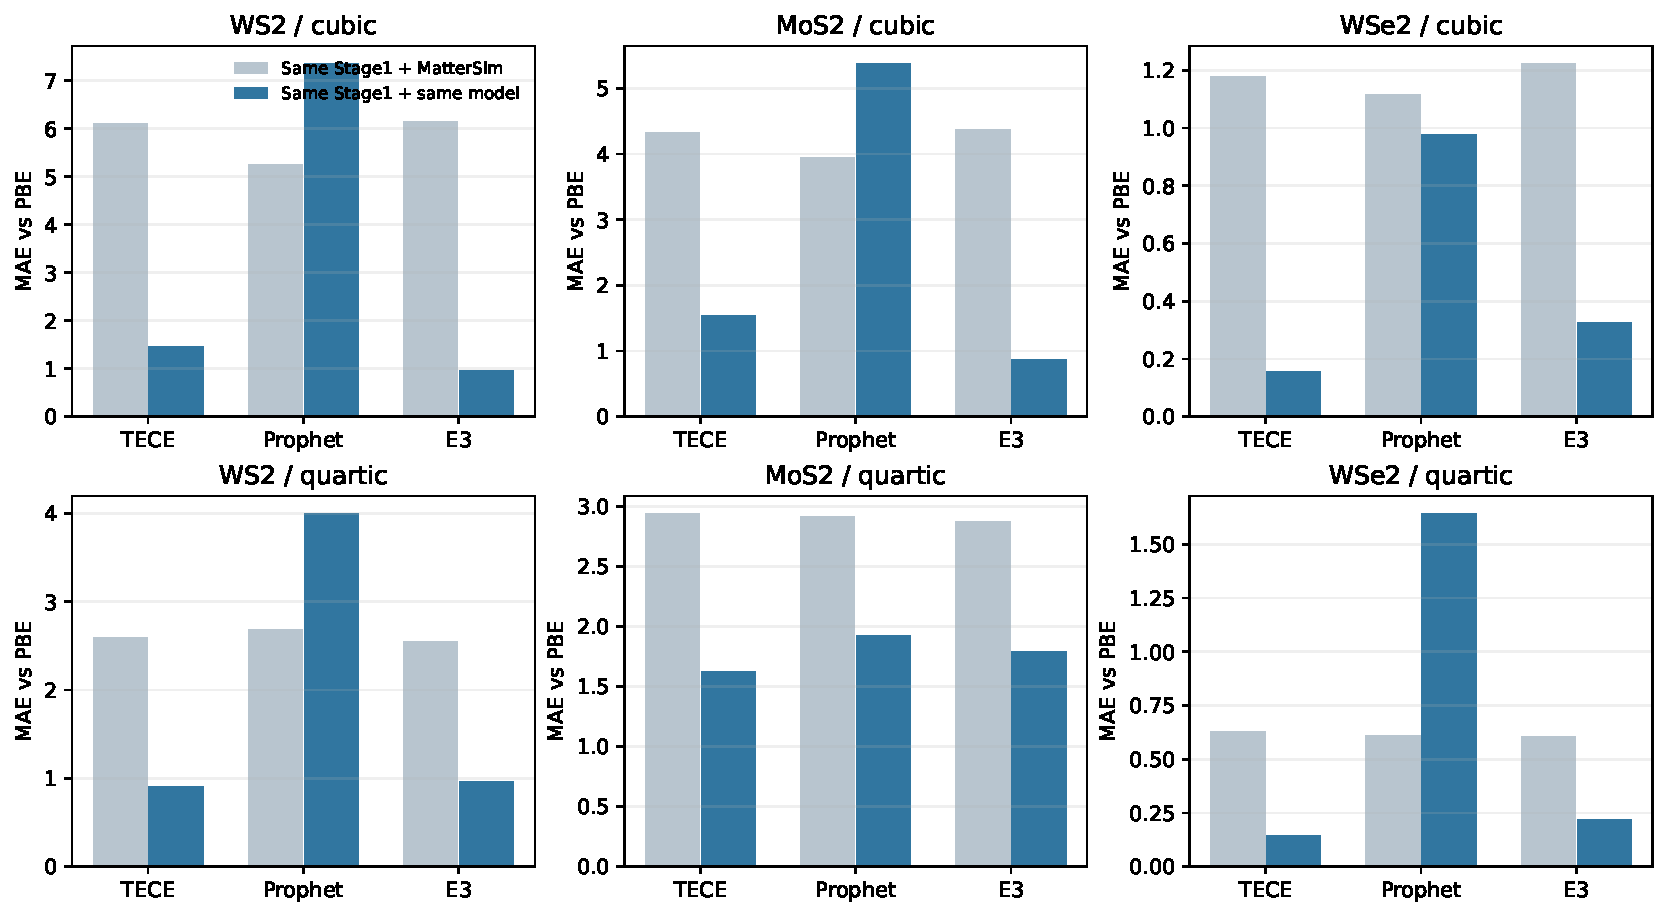
\includegraphics[width=0.98\textwidth]{figures/full_model_metrics.pdf}
\caption{复用完全相同的Stage1结构和模式后，更换Stage2对三四阶MAE的影响。每材料仅五个既定强通道，不能推广为未筛选的全部材料误差。}\label{fig:full-model-metrics}
\end{figure}
\begin{table}[!htbp]\centering\small
\caption{固定PBE DFT构型的能量／力误差：能量单位meV/超胞，力单位eV/\AA；完整181点与中心125点分开报告。}\label{tab:full-model-ef}
\allwidthtable{full_model_ef}
\end{table}
\begin{table}[!htbp]\centering\small
\caption{全流程Stage2曲率频率、中心拟合残差及首通道窗口诊断；曲率频率与匹配的PBE DFPT模式频率比较，五个Gamma和五个有限q项均保留。}
\allwidthtable{full_model_diagnostics}
\end{table}
\begin{figure}[!htbp]\centering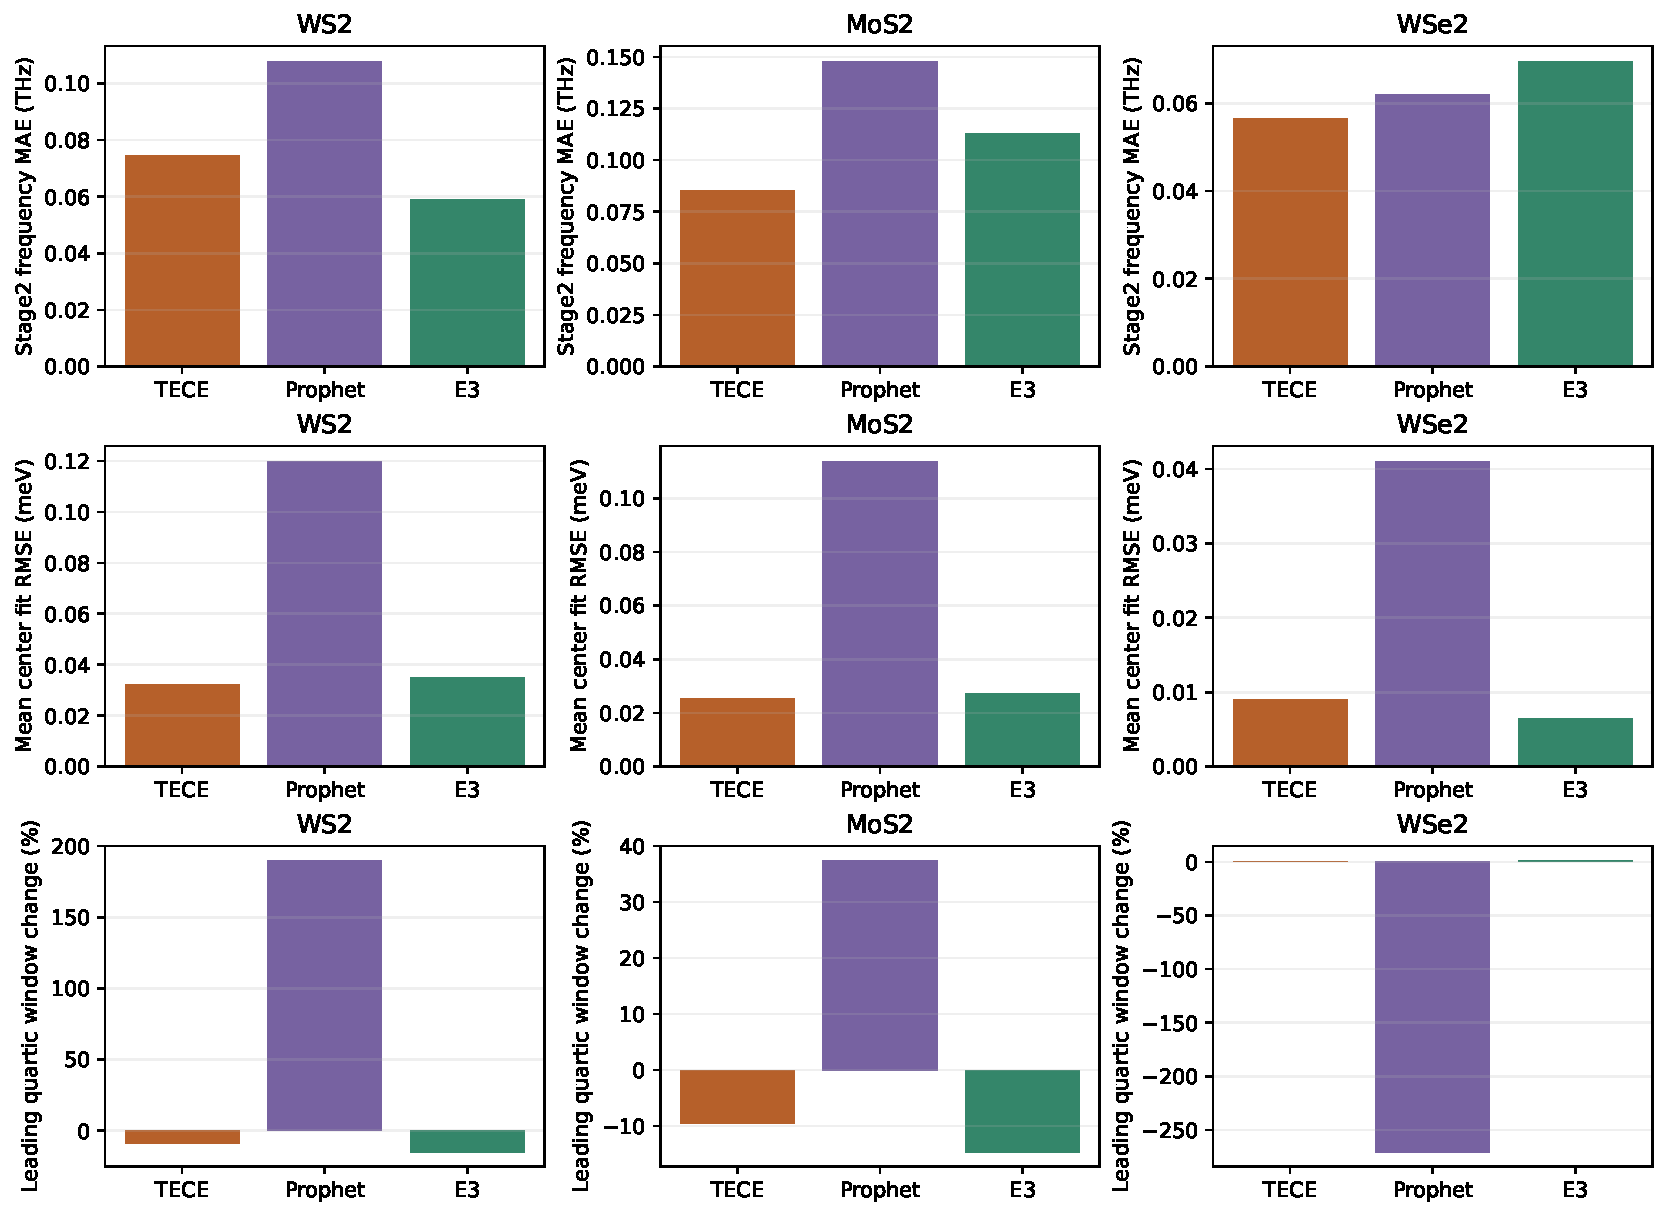
\includegraphics[width=0.98\textwidth]{figures/full_model_diagnostics.pdf}
\caption{全流程Stage2曲率频率误差、中心拟合残差及首通道四阶窗口变化。对应Stage1频率已由此前完整6$\times$6比较给出。}\label{fig:full-model-diagnostics}
\end{figure}
\begin{figure}[!htbp]\centering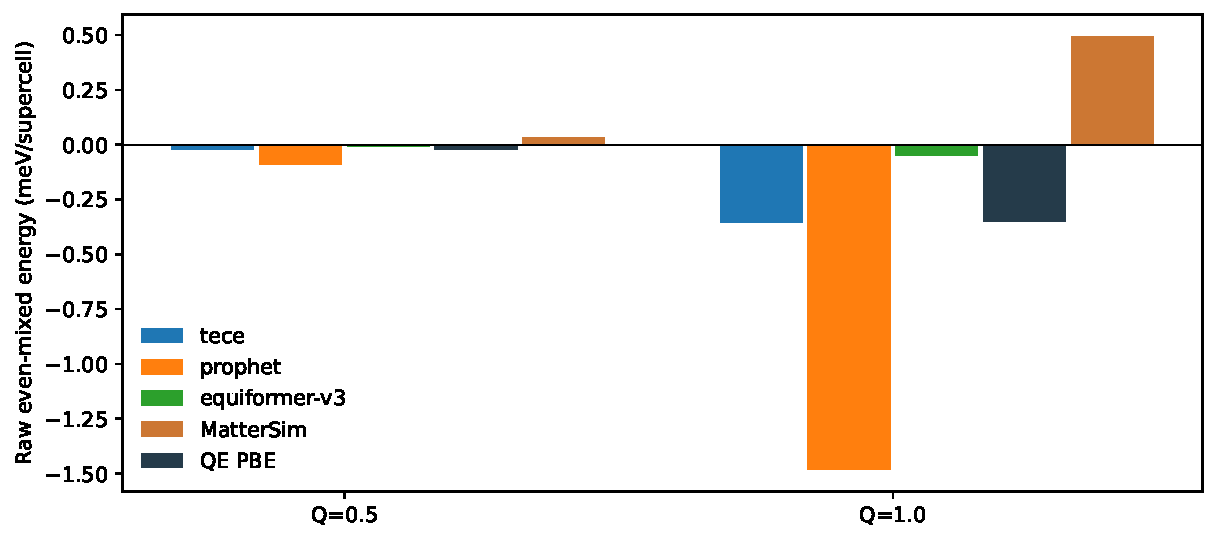
\includegraphics[width=0.9\textwidth]{figures/full_model_m6.pdf}
\caption{WS$_2$ $\Gamma8$--M6固定PBE构型的偶混合能量差。直接由原始能量消去轴向项及奇次项，不经多项式拟合。}\label{fig:full-model-m6}
\end{figure}
在这十五个固定通道内，TECE全流程相对PBE的三阶MAE在WS$_2$、MoS$_2$和WSe$_2$中分别为1.468、1.546和0.157，四阶分别为0.911、1.626和0.145。对应TECE Stage1 + MatterSim的三阶为6.104、4.328和1.180，四阶为2.594、2.939和0.628，全流程路线均有改善。EquiformerV3全流程的WS$_2$与MoS$_2$三阶MAE更低（0.953和0.868），但TECE在这三材料的四阶MAE更低；WSe$_2$的TECE全流程三四阶均表现较好。Prophet全流程并未普遍改善：WS$_2$四阶MAE为3.996、WSe$_2$为1.643，均高于对应Prophet+MatterSim。因此不能从Stage1表现推定其Stage2高阶精度，也不能把“大模型”合并为同一准确性类别。

固定PBE构型的WS$_2$ $\Gamma8$--M6中，QE四阶为$-1.4141$，TECE为$-1.4250$，MatterSim为$+1.9304$，Prophet为$-5.3944$，EquiformerV3为$-0.1993$ $\quartunit$。在$Q=1$时，不经拟合的偶混合原始能量分别为QE $-0.35252$、TECE $-0.35477$、MatterSim $+0.49472$、Prophet $-1.48308$、EquiformerV3 $-0.05150$ meV/超胞；$Q=0.5$同样给出TECE与QE接近的负号。由此可将此前结论收紧为\emph{MatterSim在该通道的混合非谐响应存在偏差}，而非MLFF普遍无法识别四阶符号。Prophet虽同号却过强；EquiformerV3虽在DFT基上同号却过弱，其自行弛豫模式基上接近零且为正（0.0299），提示近零通道仍对结构／模式选择敏感。

较好的四阶精度未必伴随较低的整张势能面能量MAE。例如MoS$_2$固定DFT构型的MatterSim能量MAE为42.849 meV，而TECE为46.134 meV；但TECE五通道四阶MAE为1.803，低于MatterSim的3.302。整体能量误差可能由谐波或轴向项主导，目标混合四阶仍须单独评价。表中原子力误差也作为独立指标保留。

现阶段可将TECE和EquiformerV3的Stage2作为更高精度的候选对照，MatterSim保留为快速筛选基线。该判断只基于既定五通道及当前CPU配置；本轮没有对三个新增Stage2开展全部324候选的筛选排名回放，也没有新增17$\times$17密度验证。全部数值仍是指定有限窗口的拟合系数，不等同于已证明零位移Taylor导数收敛。

\FloatBarrier
